\chapter{Avaliação} \label{cap:cap6}

Este capitulo apresenta várias abordagens utilizadas para avaliar a proposta desta tese. Primeiramente, a Seção~\ref{sec:CompNCL30} apresenta a execução de experimentos para avaliar como a extensão proposta se comporta em comparação a uma implementação do reconhecimento de voz usando o Ginga-NCL padrão atual com scripts Lua. A Seção~\ref{sec:cargaNCL40} apresenta a realização de um teste de carga da capacidade de manipulação de eventos do \textit{middleware}, tratando vários eventos multimodais em diversos intervalos de tempo. A Seção~\ref{sec:performanceNCL40} apresenta os testes para avaliar se houve perda de desempenho no \textit{middleware} no tratamento do eventos sendo disparados em vários intervalos de tempo de disparos, assim como intervalos de tempo diferentes para acordar os processos de leitura do servidor MQTT. Ja na Seção~\ref{sec:cargaUsuariosNCL40} apresenta a avaliação se o tratamento de perfil de multiusuários causa algum atraso significativo ao \textit{middleware}.  Além da abordagem avaliativa, este capitulo apresenta uma seção de casos de uso onde as novas funcionalidades se fazem necessárias, alguns desses casos de uso foram implementados e executados na nova versão do \textit{middleware}.

\section{Multimodalidade}\label{sec:AvMultimodalidade}

As subseções seguintes apresentam avaliação da multimodalidade, os seja, uma análise quantitativa de como o tratamento de evento de interação multimodal esta sendo realizado pelo \textit{middleware}.

\subsection{Avaliação comparativa} \label{sec:CompNCL30}

Este seção apresenta um cenário de uso para destacar como NCL estendida suporta o desenvolvimento de uma aplicação multimídia com interação de voz por múltiplos usuários. Para tal, a seção descreve uma aplicação NCL que tem como objetivo representar um cenário em que o usuário "\textit{UO1}" controla um vídeo que faz um \textit{tour} pelo Jardim Botânico. Desta maneira, apenas o usuário "\textit{U01}" pode manipular a apresentação do vídeo. Para demonstrar a implementação do evento de voz, foi desenvolvida um aplicação que inicia um vídeo a partir do comando de "\textit{play}" dito pelo usuário "\textit{U01}". As Listagens \ref{lst:ncl_multmodalNCL30} e \ref{lst:ncl_multmodal_} apresentam o conector e o link relacionado com o início do vídeo do Jardim Botânico, ativado por comando de voz. Escritas em NCL 3.0 e NCL 4.0 respectivamente.

O exemplo da Listagem~\ref{lst:ncl_multmodalNCL30} utiliza um evento de reconhecimento de voz (\textit{voiceRecognition}) por meio do script \textit{scriptInt.lua} (linha 16), que o autor precisa desenvolver e iniciá-lo junto com a aplicação que neste caso foi feita por meio do link da linha 20. Além disso será necessário um conector do tipo \textit{onEndAttribution} com um \textit{compoudCondition} para o teste que verificará se uma \textit{string} contém a palavra que indica que o "\textit{U01}" disse "play".

\begin{lstlisting}[language=ncl,label=lst:ncl_multmodalNCL30, caption={Conector e elo para interação mutimodal em NCL 3.0}]
...
<connectorBase>
  <causalConnector id="onEndAttributionTestStart">    	
    <connectorParam name="val"/>
      <compoundCondition operator="and">
        <simpleCondition role="onEndAttribution"/>       	
	    <assessmentStatement comparator="eq">
	      <attributeAssessment role="attNodeTest" eventType="attribution" attributeType="nodeProperty"/>
	      <valueAssessment value="$\$$val"/>
	    </assessmentStatement>
	  </compoundCondition>
   	  <simpleAction role="start"/>
  </causalConnector>
</connectorBase>
...
<media id="readIntModes" src="scripts/scriptInt.lua">
  <property name="key"/> 
</media>
...
<link xconnector="onBeginStart">
  <bind role="onBegin" component="botanicalGardenImage"/>
  <bind role="start" component="readIntModes" />
</link>
<link xconnector="onEndAttributionTestStart">
  <bind role="onEndAttribution" component="readIntModes" interface = "key"/>
  <bind role="attNodeTest" component="readIntModes" interface="key">
	<bindParam name="val" value="voice_recog/U01:play"/>
  </bind>	
  <bind role="start" component="botanicalGardenVideo"/>
</link>
...
\end{lstlisting}

O exemplo da Listagem~\ref{lst:ncl_multmodal_} utiliza um evento de reconhecimento de voz (\textit{voiceRecognition}) por meio do papel pré-definido \textit{onVoiceRecognition}. Esta condição possui um atributo \textit{key} que identifica o palavra a ser captada. Ainda, o atributo \textit{user} indica que tal palavra deverá ser captada do usuário (\textit{U01}).

\begin{lstlisting}[language=ncl,label=lst:ncl_multmodal_, caption={Conector e elo para interação mutimodal em NCL estendido}]
...
<connectorBase>
   <causalConnector id="onVoiceRecognitionStart">
      <connectorParam name="key"/>
      <connectorParam name="user"/>      
      <simpleCondition role="onVoiceRecognition" key="$\$$key" user= "$\$$user"/>
      <simpleAction role="start" />
   </causalConnector>  
</connectorBase>
...
<link xconnector="onVoiceRecognitionStart">
 	<bind role="onVoiceRecognition" component="botanicalGardenImage">
  		<bindParam name="key" value="play"/>
   		<bindParam name="user" value="U01"/>
 	</bind>
 	<bind role="start" component="botanicalGardenVideo"/>
 </link> 
...
\end{lstlisting}

Para avaliar a o comportamento do evento \textit{VoiceRecognition} na extensão proposta, foram construídas três aplicações NCL derivadas do exemplo na Listagem~\ref{lst:ncl_multmodal_} \footnote{As aplicações NCL e o \textit{script} de testes podem ser acessados em http://bit.do/fHiw4}. A primeira aplicação inicia um vídeo quando for dito "\textit{play}" pelo usuário "U01". A segunda aplicação inicia automaticamente um vídeo e para este vídeo, quando for dito "\textit{stop}" pelo usuário "U01". A terceira aplicação inicia automaticamente um vídeo e pausa o vídeo, quando for dito "\textit{pause}" pelo usuário "U01". 

As aplicações foram desenvolvidas em duas versões. Primeiro na versão em NCL 4.0 proposta neste trabalho. Para executá-la, foi utilizada a versão Ginga-NCL 4.0 apresentada no Capítulo~\ref{cap:cap5}. A segunda versão das aplicações foi construída utilizando NCL 3.0 e scripts NCLua emulando o comportamento do evento \textit{VoiceRecognition}.

Em todos os testes, a forma de disparar o evento de interação por voz foi simplificada para que o teste não fosse comprometido com o retardo de reconhecimento da API na nuvem da Google. Desta forma, foi produzido um script que inicia a aplicação e publica um texto no tópico \textit{voiceRecognition} de um \textit{broker} MQTT rodando na mesma máquina que o \textit{middleware} Ginga. A publicação no tópico \textit{voiceRecognition} sinaliza que algo foi dito.

Após a publicação no tópico, o \textit{VoiceRecognitionModule} deve perceber uma atualização no tópico. A partir deste momento, na versão 4.0 da classe implementada seguindo a arquitetura apresentada no Capítulo~\ref{cap:cap5} notifica o formatador sobre o evento de reconhecimento de voz. 

Na versão das aplicações em NCL 3.0, foi implementado um script NCLua que acessa o tópico MQTT desejado e dispara um evento de atribuição na aplicação NCL, que por sua vez possui links para sincronizar a atribuição com uma ação no vídeo.

Cada aplicação foi construída para testar e medir o tempo gasto desde o reconhecimento de voz até o inicio de alguma de três ações ("start", "stop" e "pause"). Experimentos foram executados com cada uma das aplicações a fim de avaliar e comparar o tempo de resposta da proposta de NCL 4.0 e de uma aplicação NCL 3.0 com \textit{scripts} Lua. Os resultados foram obtidos de uma média de 100 execuções. Os experimentos foram realizados em uma máquina com as seguintes configurações: Intel$^{\tiny{\textregistered}}$ Core™ i5-7500T CPU @ 2.70GHz; 8GB RAM; 1TB HD e Sistema Operacional Ubuntu 18.

O tempo médio ($T$) calculado em cada  experimento é definido por: 
\[ T = \sum_{i=1}^{100}{\frac{mqttPub_i+responseTime_i}{100}}\]

Onde $mqttPub$ é o tempo de comunicação entre a postagem de dados no tópico do broker, o processamento do \textit{broker} e a percepção de atualização deste tópico pelo cliente MQTT. $responseTime$ é o tempo que o Ginga demora para executar a ação esperada a partir do momento em que é reconhecida a publicação no tópico MQTT.

Na Figura~\ref{fig:grafAvaliacao}, são apresentados os resultados de experimentos para as três aplicações em suas duas versões com intervalo de confiança de 95\%. Na cor azul, é apresentado o tempo médio das aplicações criadas com NCL 4.0. Na cor verde, pode-se observar o tempo médio das aplicações criadas com NCL 3.0 e scripts NCLua. Pode-se observar que a aplicação com a proposta deste trabalho com NCL 4.0 possui tempo de resposta abaixo de 70$ms$ enquanto todas as aplicações feitas em NCL 3.0 superam 200$ms$ para responder a ação. 

\begin{figure}[h!]
    \centering
    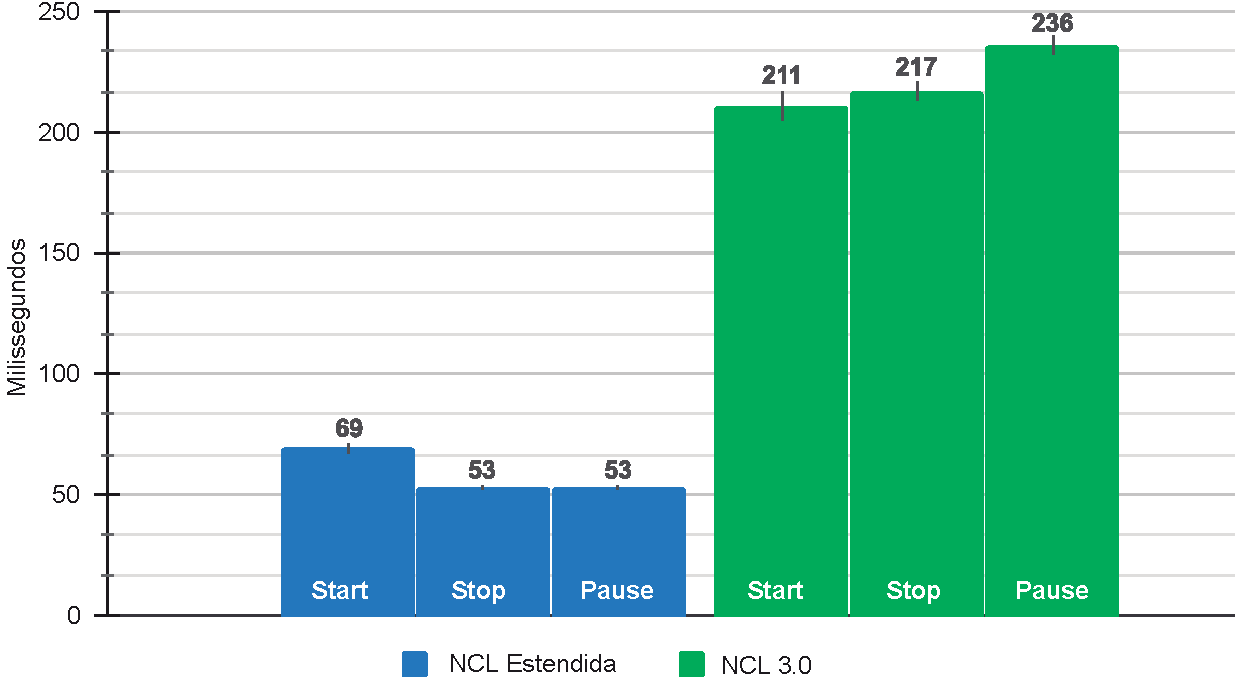
\includegraphics[scale=0.5, keepaspectratio=true]{figuras/graficoAvaliacao1.pdf}
    \caption{Média de tempo (ms) gasto para aplicação reagir a uma publicação MQTT de start/stop/pause em uma mídia.}
    \label{fig:grafAvaliacao}
\end{figure}

Como pode ser visto na Figura~\ref{fig:grafAvaliacao}, o tempo de resposta de uma aplicação em NCL 4.0 é aproximadamente um terço do tempo de uma aplicação feita utilizando NCL 3.0 e Lua. Além disso, em NCL 4.0, o autor da aplicação não precisa programar em uma linguagem imperativa e não precisa acoplar módulos ou scripts NCLua à sua aplicação existente. Estes resultados demonstram que a implementação de interação multimodal proposta no Ginga oferece bom desempenho.

Com o uso de NCL 4.0, também há uma diminuição do esforço de autoria. O autor da aplicação, usando NCL 4.0, deve declarar apenas $1$ conector e $1$ link para prover a interação por voz. A aplicação tem um total de $49$ linhas de código para descrever seu comportamento. Por outro lado, em NCL 3.0, o autor necessita de scripts NCLua para realizar o acesso aos tópicos MQTT e criação de um conector de atribuição para emular um evento de reconhecimento de voz. A aplicação NCL 3.0 tem um total de $158$ linhas de código.

Adicionalmente, a forma de descrever interação multimodal por meio de eventos da linguagem NCL favorece a legibilidade do código NCL. Pois quando o usuário define um conector com o papel \textit{onVoiceRecognition}, é mais fácil de entender que se trata de um reconhecimento de voz do que ter que criar um conector com papel  \textit{onEndAtribution} para tratar o evento de reconhecimento de voz gerado pelo \textit{script} Lua.

\subsection{Avaliação de carga} \label{sec:cargaNCL40}

Para avaliar a capacidade do \textit{middleware} de lidar com inúmeros eventos multimodais, esta seção apresenta vários testes realizados que usaram várias aplicações NCL simples. Essas aplicações possuíam links que eram disparados com eventos de interação por meio de voz e gesto. As interações foram representadas no teste por meio de publicações em tópicos MQTT onde os dispositivos responsáveis por essas interações multimodais publicam. Isso foi possível por causa da execução de um \textit{script} fazendo as publicações. O \textit{middleware} ouviu  esses tópicos por meio dos módulos de interação (IMs). Sempre que ocorreu uma publicação, os IMs sinalizaram para o \textit{middleware}, que por sua vez sinalizou para todos objetos interessados nos eventos na aplicação NCL. Assim, o teste utilizou uma aplicação NCL que alterava uma variável cada vez que uma publicação era recebida, ou seja, para confirmar que a ação aconteceu e que o evento foi capturado. Para avaliar esse comportamento, a aplicação foi executada com os módulos do \textit{middleware} ouvindo eventos a cada 10 milissegundos. Este é um parâmetro do Ginga que pode ser configurado. O teste emulou 100 eventos disparados em intervalos de 10$ms$; 15$ms$; 20$ms$; 30$ms$; 40$ms$ e 50$ms$ e contou quantos eventos foram capturados e manipulados para cada valor de intervalo. O teste repetiu esse processo 100 vezes e, em seguida, calculamos a média de cada intervalo. A Figura~\ref{fig:grafAvaliacao2} mostra os resultados obtidos. Podemos ver que, para os intervalos de 20$ms$ e superiores, o Ginga obteve uma excelente taxa de captura de eventos, atingindo em média 99,9\% de capturas.
\begin{figure}[h!]
    \centering
    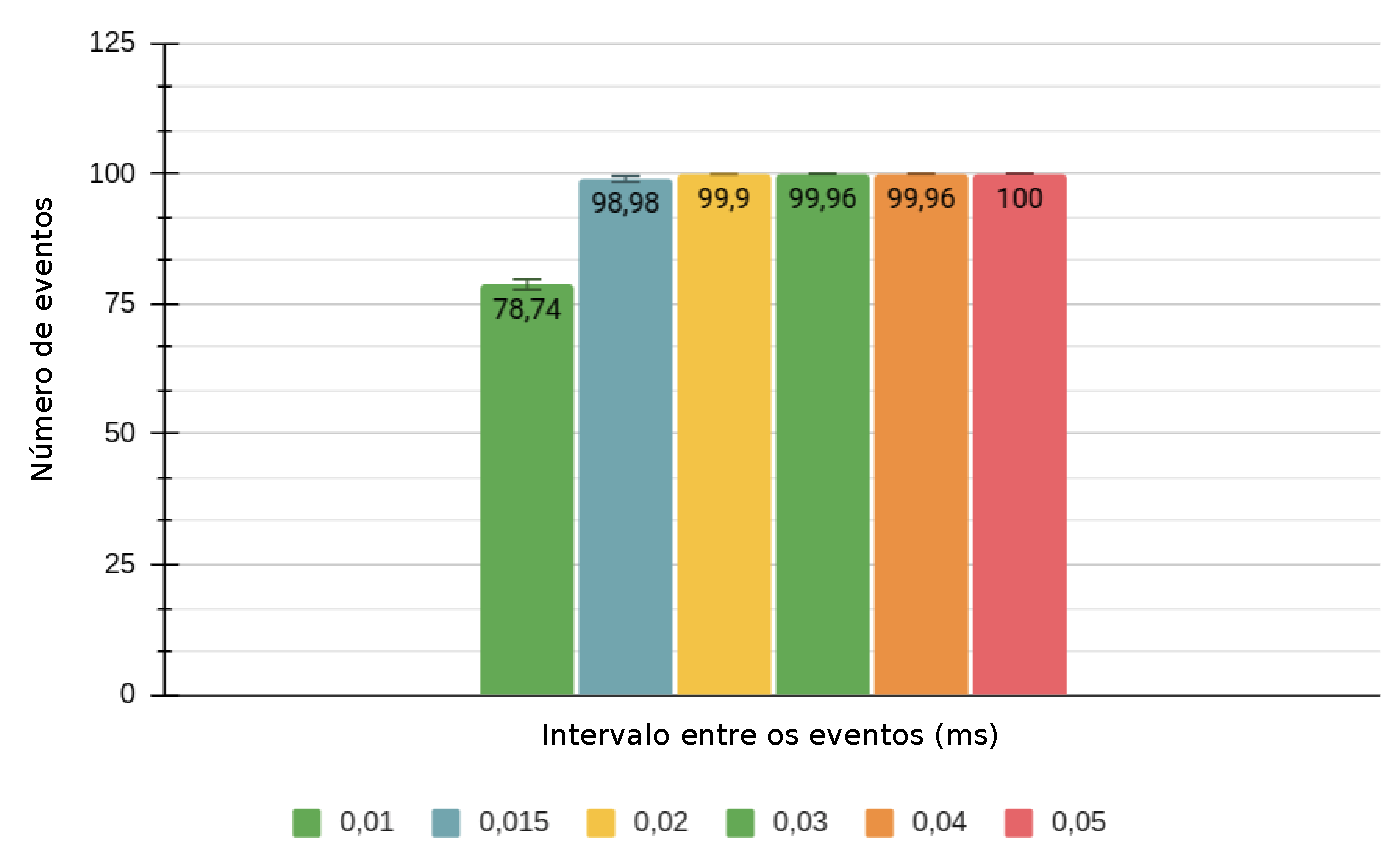
\includegraphics[scale=0.50, keepaspectratio=true]{figuras/grafEventosCap.pdf}
    \caption{Média do número de eventos capturados}
    \label{fig:grafAvaliacao2}
\end{figure}


\subsection{Avaliação de performance} \label{sec:performanceNCL40}

Neste experimento, o teste avalia o quanto esse tratamento de novos eventos retarda a extensão do \textit{middleware} proposta. Para isso, primeiramente o teste mediu o atraso causado pela escuta dos módulos sem acionar os eventos e depois ouvindo o acionamento do evento. O teste utilizou \textit{scripts} que realizaram essas publicações MQTT em intervalos de 20\textit{ms}, que é o menor intervalo com 99,9\% dos eventos capturados, conforme encontrado na Figura~\ref{fig:grafAvaliacao2}. Para isso, uma aplicação NCL foi criada com uma imagem de fundo com âncoras temporais que iniciaram quatro outras imagens. Para cada segundo, uma nova imagem foi iniciada. A visão temporal deste aplicativo é mostrada na Figura~\ref{fig:timeView}. A aplicação foi executada 100 vezes, e o teste calculou a média do tempo de início de cada imagem associada às âncoras temporais. Essas execuções foram feitas em três cenários diferentes: 

             (1) Rodar a aplicação sem os IMs (Ginga-NCL estendido sem iniciar os IMs);
             
             (2) Rodar a aplicação com os IMs sem receber eventos de interação (IMs iniciados com Ginga-NCL estendido);
             
             (3) Executar a aplicação com os IMs e receber 300 eventos de interação (150 eventos de reconhecimento de voz e 150 gestos) (Ginga-NCL estendido iniciando e sobrecarregando IMs).

\begin{figure}[h!]
    \centering
    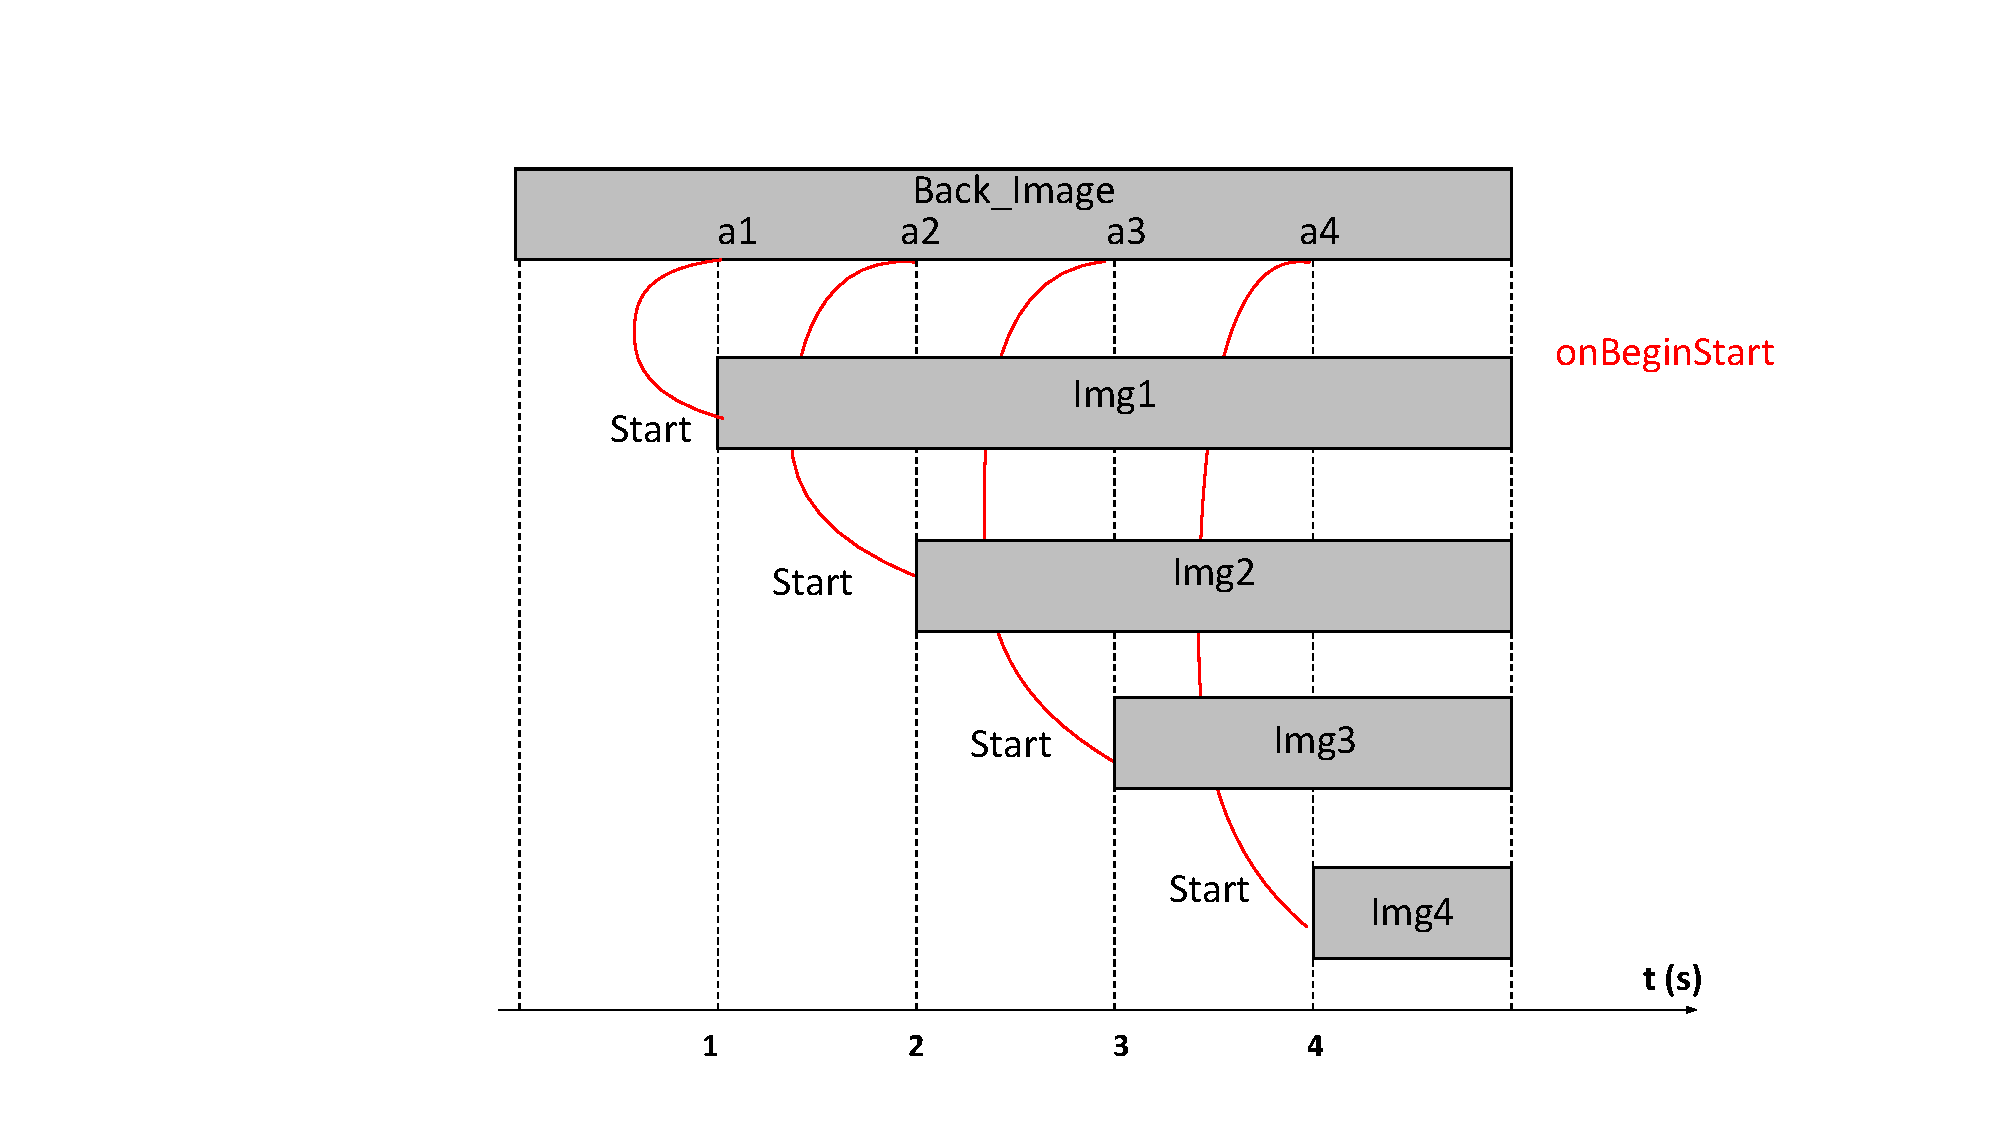
\includegraphics[scale=0.50, keepaspectratio=true]{figuras/VisaoTemporalAppCarga.pdf}
    \caption{Visão Temporal da aplicação usada para avaliar o atraso em três diferentes cenários}
    \label{fig:timeView}
\end{figure}

A Figura~\ref{fig:average} mostra o atraso médio da apresentação de cada objeto de mídia nesses três cenários diferentes. Observe que nos cenários (2) e (3), o \textit{middleware} desperta o ouvinte a cada 10$ms$. No cenário (2), podemos observar que o ouvinte, sem disparar os eventos causa um atraso da ordem de 9$ms$. No cenário (3), o disparo de 300 eventos no intervalo de 20$ms$, com os módulos acordando e ouvindo a cada 10$ms$.
Podemos ver na Figura~\ref{fig:average} que a extensão proposta não impacta o \textit{middleware} Ginga quando nenhum ouvinte de evento multimodal está ativo. Além disso, para o cenário (2) o atraso médio resultante foi de $\approx$ 6$ms$ e para o cenário (3) o atraso médio foi de $\approx$ 11$ms$. A implementação de nossos ouvintes adiciona pelo menos um atraso de $\approx$ 6$ms$ na implementação estendida do Ginga-NCL; no entanto, esse atraso não aumenta à medida que o número de eventos aumenta. Além disso, o pior caso de atraso no cenário (3) foi de 13$ms$ em \textit{img1}. De acordo com o trabalho de Card et. al \cite{card1986model}, leva 230 $ms$ para um humano perceber algo visualmente. Assim, como nosso pior cenário adiciona à percepção de \textit{img1} um atraso de $\approx \frac{1}{17}$ do tempo identificado em \cite{card1986model}, ele não representa um impacto na apresentação de \textit{img1}.

\begin{figure}[h!]
    \centering
    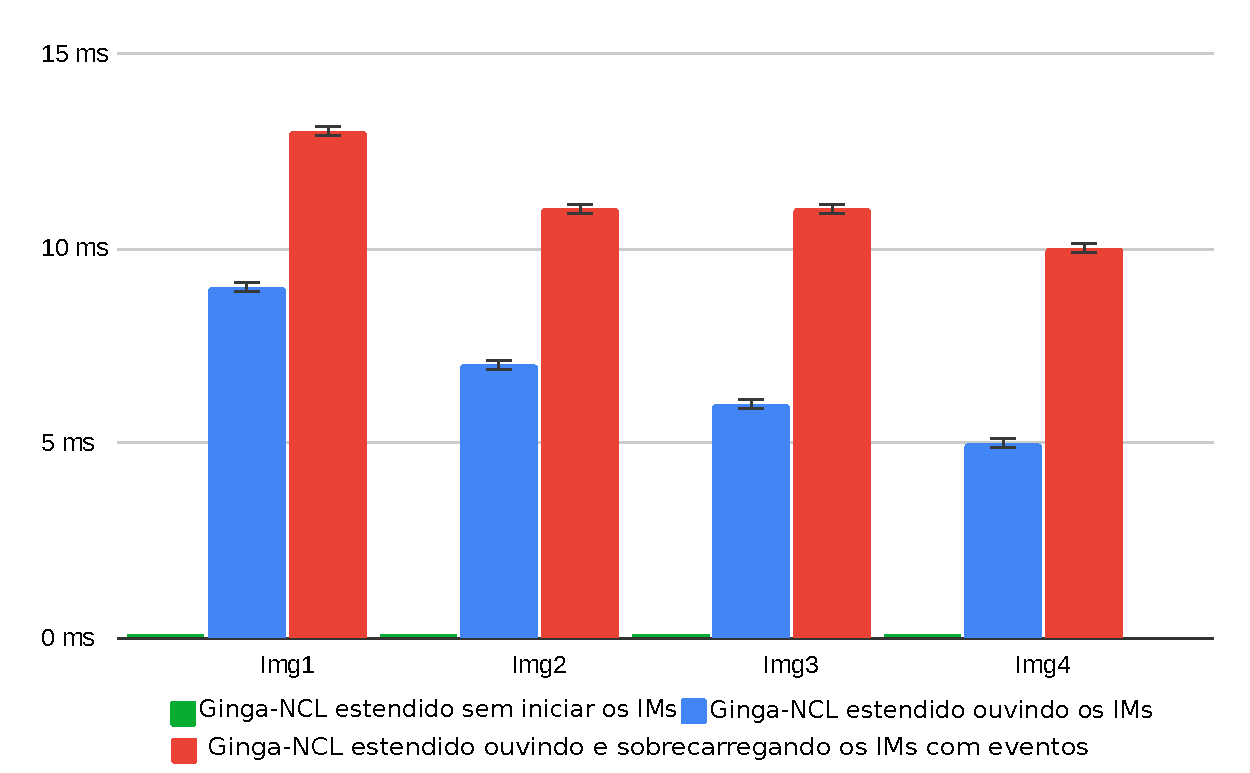
\includegraphics[scale=0.60, keepaspectratio=true]{figuras/scenarios.pdf}
    \caption{Média de atraso (em ms) de cada mídia na aplicação para cada cenário}
    \label{fig:average}
\end{figure}


\section{Multiusuário}\label{sec:AvMultiusuario}

Esta seção apresenta avaliação de multiusuário, ou seja, uma análise quantitativa de como \textit{middleware} se comporta com o tratamento das funcionalidades para uma aplicação multiusuário especificadas neste trabalho. Para isso, esta seção apresenta a avaliação em duas partes. A primeira mede tempo gasto no reconhecimento dos usuários cujo propriedades estão armazenadas em arquivos XML. A maior processamento acontece quando a aplicação tem um perfil a ser validado. Pois conforme foi dito no Capitulo~\ref{cap:cap4}, quando a aplicação tem algum \textit{userProfile}, todas as propriedades são comparadas com as propriedades de todos os usuários que estão armazenados no \textit{setbox}. Assim, somente os usuários que tenha tais propriedades, irão ter suas interações consideradas pelo \textit{middleware}. A segunda parte mede o tempo gasto para criação de todos o links dinâmicos a partir dos usuários encontrados e que atendam o perfil.

Os resultados foram obtidos de uma média de 100 execuções. Os experimentos foram realizados em uma máquina com as seguintes configurações: Intel$^{\tiny{\textregistered}}$ Core™ i5-7500T CPU @ 2.70GHz; 8GB RAM; 1TB HD e Sistema Operacional Ubuntu 18.

Na primeira parte cada aplicação foi construída para testar e medir o tempo gasto para reconhecer de todos os usuários com o perfil especificado na aplicação. Para isso, o experimento usou 5 cenários onde varia o número de usuários e de propriedades comparadas com as propriedades do perfil usado. A Tabela~\ref{tab:expUserPerfil} apresenta os cenários com a média dos tempos gasto para carregar os usuários em 100 execuções.

\begin{table}[h]
\centering
{
  % distancia entre a linha e o texto
  \renewcommand\arraystretch{1.25}
  \begin{tabular}{|p{1,5cm}|p{6cm}|p{1,5cm}|p{2cm}|} \hline
   \multicolumn{1}{|c|}{Cenário} & \multicolumn{1}{|c|}{Descrição} & \multicolumn{1}{c|}{Média (ms)} & \multicolumn{1}{c|}{Confiança} \\\hline
    1 & 1 usuário com 5 propriedades &  0  & 1,09E-09    \\\hline
    2 & 5 usuários com 5 propriedades &  1  & 2,04E-09   \\\hline
    3 & 10 usuários com 5 propriedades &  1  & 7,76E-10  \\\hline
    4 & 5 usuários com 10 propriedades &  1  & 1,06E-09  \\\hline
    5 & 10 usuários com 10 propriedades &  1  & 1,47E-09 \\\hline
   \end{tabular}
\caption{Cenários contemplados no experimento para usuários de um perfil}
\label{tab:expUserPerfil}
}
\end{table}

Na segunda parte cada aplicação foi construída para testar e medir o tempo gasto para criar os links dinâmicos para cada usuário. Para isso, o experimento usou 9 cenários onde varia o número de usuários e de links com perfil usado. A Tabela~\ref{tab:expUserPerfil} apresenta os cenários com a média dos tempos gasto para carregar os usuários em 100 execuções.

\begin{table}[h]
\centering
{
  % distancia entre a linha e o texto
  \renewcommand\arraystretch{1.25}
  \begin{tabular}{|p{1,5cm}|p{6cm}|p{1,5cm}|p{2cm}|} \hline
   \multicolumn{1}{|c|}{Cenário} & \multicolumn{1}{|c|}{Descrição} & \multicolumn{1}{c|}{Média (ms)} & \multicolumn{1}{c|}{Confiança} \\\hline
   
   1 & 1 link com 1 user & 0 & 0 \\\hline
   2 & 10 links com 1 user & 0 & 5,89E-10 \\\hline
   3 & 50 links com 1 user & 0 & 9,40E-10 \\\hline	 	
   
   4 & 1 link com 5 users & 0 & 3,94E-10 \\\hline
   5 & 10 links com 5 users & 0 & 6,61E-10 \\\hline	
   6 & 50 links com 5 users & 1 & 1,59E-09 \\\hline		

   7 & 1 link com 10 users & 0 & 3,94E-10   \\\hline
   8 & 10 links com 10 users & 0 & 1,12E-09 \\\hline	
   9 & 50 links com 10 users & 5 &  4,11E-09 \\\hline		
 
   \end{tabular}
\caption{Cenários contemplados no experimento para criação de links de um perfil}
\label{tab:expLinksPerfil}
}
\end{table}

Como mostra as Tabelas ~\ref{tab:expUserPerfil} e ~\ref{tab:expLinksPerfil} o tempo gasto no pior caso do experimento, ainda se mostra excelente pois fazendo somatório do tempo para carregar 10 usuários contendo 10 propriedades comparadas mais o tempo gasto em uma aplicação com 50 links, o total é de 6 ms durante a carregamento da aplicação, ou seja, antes da apresentação das mídias.

Este capitulo apresentou a avaliação da proposta desta tese quanto ao uso de várias modalidades de interação. Esta avaliação foi feita em três abordagens: Comparativa, carga e performance. E também a avaliação de aplicações multiusuário em duas partes duas, reconhecimentos dos usuários e carga da criação de links dinâmicos.

